% Options for packages loaded elsewhere
% Options for packages loaded elsewhere
\PassOptionsToPackage{unicode}{hyperref}
\PassOptionsToPackage{hyphens}{url}
\PassOptionsToPackage{dvipsnames,svgnames,x11names}{xcolor}
%
\documentclass[
  letterpaper,
  DIV=11,
  numbers=noendperiod]{scrreprt}
\usepackage{xcolor}
\usepackage{amsmath,amssymb}
\setcounter{secnumdepth}{5}
\usepackage{iftex}
\ifPDFTeX
  \usepackage[T1]{fontenc}
  \usepackage[utf8]{inputenc}
  \usepackage{textcomp} % provide euro and other symbols
\else % if luatex or xetex
  \usepackage{unicode-math} % this also loads fontspec
  \defaultfontfeatures{Scale=MatchLowercase}
  \defaultfontfeatures[\rmfamily]{Ligatures=TeX,Scale=1}
\fi
\usepackage{lmodern}
\ifPDFTeX\else
  % xetex/luatex font selection
\fi
% Use upquote if available, for straight quotes in verbatim environments
\IfFileExists{upquote.sty}{\usepackage{upquote}}{}
\IfFileExists{microtype.sty}{% use microtype if available
  \usepackage[]{microtype}
  \UseMicrotypeSet[protrusion]{basicmath} % disable protrusion for tt fonts
}{}
\makeatletter
\@ifundefined{KOMAClassName}{% if non-KOMA class
  \IfFileExists{parskip.sty}{%
    \usepackage{parskip}
  }{% else
    \setlength{\parindent}{0pt}
    \setlength{\parskip}{6pt plus 2pt minus 1pt}}
}{% if KOMA class
  \KOMAoptions{parskip=half}}
\makeatother
% Make \paragraph and \subparagraph free-standing
\makeatletter
\ifx\paragraph\undefined\else
  \let\oldparagraph\paragraph
  \renewcommand{\paragraph}{
    \@ifstar
      \xxxParagraphStar
      \xxxParagraphNoStar
  }
  \newcommand{\xxxParagraphStar}[1]{\oldparagraph*{#1}\mbox{}}
  \newcommand{\xxxParagraphNoStar}[1]{\oldparagraph{#1}\mbox{}}
\fi
\ifx\subparagraph\undefined\else
  \let\oldsubparagraph\subparagraph
  \renewcommand{\subparagraph}{
    \@ifstar
      \xxxSubParagraphStar
      \xxxSubParagraphNoStar
  }
  \newcommand{\xxxSubParagraphStar}[1]{\oldsubparagraph*{#1}\mbox{}}
  \newcommand{\xxxSubParagraphNoStar}[1]{\oldsubparagraph{#1}\mbox{}}
\fi
\makeatother

\usepackage{color}
\usepackage{fancyvrb}
\newcommand{\VerbBar}{|}
\newcommand{\VERB}{\Verb[commandchars=\\\{\}]}
\DefineVerbatimEnvironment{Highlighting}{Verbatim}{commandchars=\\\{\}}
% Add ',fontsize=\small' for more characters per line
\usepackage{framed}
\definecolor{shadecolor}{RGB}{241,243,245}
\newenvironment{Shaded}{\begin{snugshade}}{\end{snugshade}}
\newcommand{\AlertTok}[1]{\textcolor[rgb]{0.68,0.00,0.00}{#1}}
\newcommand{\AnnotationTok}[1]{\textcolor[rgb]{0.37,0.37,0.37}{#1}}
\newcommand{\AttributeTok}[1]{\textcolor[rgb]{0.40,0.45,0.13}{#1}}
\newcommand{\BaseNTok}[1]{\textcolor[rgb]{0.68,0.00,0.00}{#1}}
\newcommand{\BuiltInTok}[1]{\textcolor[rgb]{0.00,0.23,0.31}{#1}}
\newcommand{\CharTok}[1]{\textcolor[rgb]{0.13,0.47,0.30}{#1}}
\newcommand{\CommentTok}[1]{\textcolor[rgb]{0.37,0.37,0.37}{#1}}
\newcommand{\CommentVarTok}[1]{\textcolor[rgb]{0.37,0.37,0.37}{\textit{#1}}}
\newcommand{\ConstantTok}[1]{\textcolor[rgb]{0.56,0.35,0.01}{#1}}
\newcommand{\ControlFlowTok}[1]{\textcolor[rgb]{0.00,0.23,0.31}{\textbf{#1}}}
\newcommand{\DataTypeTok}[1]{\textcolor[rgb]{0.68,0.00,0.00}{#1}}
\newcommand{\DecValTok}[1]{\textcolor[rgb]{0.68,0.00,0.00}{#1}}
\newcommand{\DocumentationTok}[1]{\textcolor[rgb]{0.37,0.37,0.37}{\textit{#1}}}
\newcommand{\ErrorTok}[1]{\textcolor[rgb]{0.68,0.00,0.00}{#1}}
\newcommand{\ExtensionTok}[1]{\textcolor[rgb]{0.00,0.23,0.31}{#1}}
\newcommand{\FloatTok}[1]{\textcolor[rgb]{0.68,0.00,0.00}{#1}}
\newcommand{\FunctionTok}[1]{\textcolor[rgb]{0.28,0.35,0.67}{#1}}
\newcommand{\ImportTok}[1]{\textcolor[rgb]{0.00,0.46,0.62}{#1}}
\newcommand{\InformationTok}[1]{\textcolor[rgb]{0.37,0.37,0.37}{#1}}
\newcommand{\KeywordTok}[1]{\textcolor[rgb]{0.00,0.23,0.31}{\textbf{#1}}}
\newcommand{\NormalTok}[1]{\textcolor[rgb]{0.00,0.23,0.31}{#1}}
\newcommand{\OperatorTok}[1]{\textcolor[rgb]{0.37,0.37,0.37}{#1}}
\newcommand{\OtherTok}[1]{\textcolor[rgb]{0.00,0.23,0.31}{#1}}
\newcommand{\PreprocessorTok}[1]{\textcolor[rgb]{0.68,0.00,0.00}{#1}}
\newcommand{\RegionMarkerTok}[1]{\textcolor[rgb]{0.00,0.23,0.31}{#1}}
\newcommand{\SpecialCharTok}[1]{\textcolor[rgb]{0.37,0.37,0.37}{#1}}
\newcommand{\SpecialStringTok}[1]{\textcolor[rgb]{0.13,0.47,0.30}{#1}}
\newcommand{\StringTok}[1]{\textcolor[rgb]{0.13,0.47,0.30}{#1}}
\newcommand{\VariableTok}[1]{\textcolor[rgb]{0.07,0.07,0.07}{#1}}
\newcommand{\VerbatimStringTok}[1]{\textcolor[rgb]{0.13,0.47,0.30}{#1}}
\newcommand{\WarningTok}[1]{\textcolor[rgb]{0.37,0.37,0.37}{\textit{#1}}}

\usepackage{longtable,booktabs,array}
\usepackage{calc} % for calculating minipage widths
% Correct order of tables after \paragraph or \subparagraph
\usepackage{etoolbox}
\makeatletter
\patchcmd\longtable{\par}{\if@noskipsec\mbox{}\fi\par}{}{}
\makeatother
% Allow footnotes in longtable head/foot
\IfFileExists{footnotehyper.sty}{\usepackage{footnotehyper}}{\usepackage{footnote}}
\makesavenoteenv{longtable}
\usepackage{graphicx}
\makeatletter
\newsavebox\pandoc@box
\newcommand*\pandocbounded[1]{% scales image to fit in text height/width
  \sbox\pandoc@box{#1}%
  \Gscale@div\@tempa{\textheight}{\dimexpr\ht\pandoc@box+\dp\pandoc@box\relax}%
  \Gscale@div\@tempb{\linewidth}{\wd\pandoc@box}%
  \ifdim\@tempb\p@<\@tempa\p@\let\@tempa\@tempb\fi% select the smaller of both
  \ifdim\@tempa\p@<\p@\scalebox{\@tempa}{\usebox\pandoc@box}%
  \else\usebox{\pandoc@box}%
  \fi%
}
% Set default figure placement to htbp
\def\fps@figure{htbp}
\makeatother





\setlength{\emergencystretch}{3em} % prevent overfull lines

\providecommand{\tightlist}{%
  \setlength{\itemsep}{0pt}\setlength{\parskip}{0pt}}



 


\KOMAoption{captions}{tableheading}
\makeatletter
\@ifpackageloaded{bookmark}{}{\usepackage{bookmark}}
\makeatother
\makeatletter
\@ifpackageloaded{caption}{}{\usepackage{caption}}
\AtBeginDocument{%
\ifdefined\contentsname
  \renewcommand*\contentsname{Table of contents}
\else
  \newcommand\contentsname{Table of contents}
\fi
\ifdefined\listfigurename
  \renewcommand*\listfigurename{List of Figures}
\else
  \newcommand\listfigurename{List of Figures}
\fi
\ifdefined\listtablename
  \renewcommand*\listtablename{List of Tables}
\else
  \newcommand\listtablename{List of Tables}
\fi
\ifdefined\figurename
  \renewcommand*\figurename{Figure}
\else
  \newcommand\figurename{Figure}
\fi
\ifdefined\tablename
  \renewcommand*\tablename{Table}
\else
  \newcommand\tablename{Table}
\fi
}
\@ifpackageloaded{float}{}{\usepackage{float}}
\floatstyle{ruled}
\@ifundefined{c@chapter}{\newfloat{codelisting}{h}{lop}}{\newfloat{codelisting}{h}{lop}[chapter]}
\floatname{codelisting}{Listing}
\newcommand*\listoflistings{\listof{codelisting}{List of Listings}}
\makeatother
\makeatletter
\makeatother
\makeatletter
\@ifpackageloaded{caption}{}{\usepackage{caption}}
\@ifpackageloaded{subcaption}{}{\usepackage{subcaption}}
\makeatother
\usepackage{bookmark}
\IfFileExists{xurl.sty}{\usepackage{xurl}}{} % add URL line breaks if available
\urlstyle{same}
\hypersetup{
  pdftitle={EL-2007 Sinyal dan Sistem},
  pdfauthor={Armein Z R Langi},
  colorlinks=true,
  linkcolor={blue},
  filecolor={Maroon},
  citecolor={Blue},
  urlcolor={Blue},
  pdfcreator={LaTeX via pandoc}}


\title{EL-2007 Sinyal dan Sistem}
\author{Armein Z R Langi}
\date{2025-09-03}
\begin{document}
\maketitle

\renewcommand*\contentsname{Table of contents}
{
\hypersetup{linkcolor=}
\setcounter{tocdepth}{2}
\tableofcontents
}

\bookmarksetup{startatroot}

\chapter*{Selamat Datang di KuLiahEL 2007 Sinyal dan
Sistem}\label{selamat-datang-di-kuliahel-2007-sinyal-dan-sistem}
\addcontentsline{toc}{chapter}{Selamat Datang di KuLiahEL 2007 Sinyal
dan Sistem}

\markboth{Selamat Datang di KuLiahEL 2007 Sinyal dan Sistem}{Selamat
Datang di KuLiahEL 2007 Sinyal dan Sistem}

Video Clip
\url{https://www.youtube.com/playlist?list=PLgnoib8dkAOy1CnW9UXWDRpcdEpDVWfey}

This is a Quarto book.

To learn more about Quarto books visit
\url{https://quarto.org/docs/books}.

\bookmarksetup{startatroot}

\chapter{Capaian Belajar}\label{capaian-belajar}

Berikut adalah rancangan pembelajaran satu semester untuk mata kuliah
\textbf{Sinyal dan Sistem (EL2007)}, yang telah ditambahkan dengan
rujukan pada buku teks \emph{Signals and Systems} oleh Oppenheim dan
\emph{Schaum's Outline of Signals and Systems} oleh Hwei Hsu.

\textbf{Rencana Pembelajaran Satu Semester}

\textbf{Kode Mata Kuliah:} EL2007 \textbf{Nama Mata Kuliah:} Sinyal dan
Sistem / Signals and Systems \textbf{Jumlah SKS:} 3 SKS
\textbf{Penyelenggara:} 132 - Teknik Elektro / STEI
\textbf{Co-requisite:} MA2074 Matematika Rekayasa IIA / Engineering
Mathematics IIA \textbf{Bahasa Pengantar:} Bahasa Indonesia / English

\textbf{Capaian Pembelajaran Mata Kuliah (CPMK):} Setelah mengikuti mata
kuliah ini, mahasiswa diharapkan mampu: 1. \textbf{Menganalisis sifat
sinyal dan sistem} dalam domain waktu, domain frekuensi, dan domain
Laplace. 2. \textbf{Merancang filter dan pengendali secara matematis}
pada studi kasus. 3. \textbf{Menggunakan alat bantu (perangkat lunak)}
untuk menganalisis sinyal dan sistem.

\textbf{Metode Pembelajaran:} Ceramah, Diskusi, Studi Kasus, Belajar
\textbf{Modalitas Pembelajaran:} Luring, Daring, Bauran (Offline,
Online, Hybrid) \textbf{Metode Penilaian:} PR (Pekerjaan Rumah), Kuis,
Ujian \textbf{Jenis Nilai:} ABCDE

\begin{center}\rule{0.5\linewidth}{0.5pt}\end{center}

\textbf{Distribusi Materi dan Kegiatan Per Minggu (14 Minggu
Perkuliahan):}

\textbf{Minggu 1:} * \textbf{Bahan Kajian:} Deskripsi Matematis Sinyal
Waktu Kontinu (Mathematical Description of Continuous-time Signals). *
\textbf{CPMK Terkait:} Memahami dasar-dasar sinyal waktu kontinu dan
representasi matematisnya. * \textbf{Kegiatan:} Ceramah dan Diskusi
tentang jenis-jenis sinyal dan operasi dasar sinyal. * \textbf{Rujukan:}
* \textbf{Oppenheim:} Bab 2 (Signals, Transformations of the Independent
Variable, Basic Continuous-Time Signals). * \textbf{Schaum's Series:}
Bab 1 (Signals and Systems, Signals and Classification of Signals, Basic
Continuous-Time Signals). Lihat juga Solved Problems seperti 1.3, 1.4,
1.5, 1.19, 1.46, 1.47, 1.48 untuk latihan.

\textbf{Minggu 2-3:} * \textbf{Bahan Kajian:} Deskripsi Sistem di Domain
Waktu: Persamaan Diferensial dan Respon Impuls (Time-Domain Description
of Systems: Differential Equation and Impulse Response). * \textbf{CPMK
Terkait:} Mengenal karakteristik sistem linear tak-berubah waktu (LTI)
dan representasinya melalui persamaan diferensial dan respon impuls. *
\textbf{Kegiatan:} Ceramah dan Diskusi mengenai konsep sistem,
sifat-sifatnya, dan pentingnya respon impuls. * \textbf{Penilaian (Akhir
Minggu 3):} PR 1 (terkait deskripsi sinyal dan sistem di domain waktu).
* \textbf{Rujukan:} * \textbf{Oppenheim:} Bab 2 (Systems, Properties of
Systems), Bab 3 (Linear Time-Invariant Systems, The Representation of
Signals in Terms of Impulses, Systems Described by Differential and
Difference Equations). * \textbf{Schaum's Series:} Bab 1 (Systems and
Classification of Systems), Bab 2 (Introduction, Systems Described by
Differential Equations, Eigenfunctions of Continuous-Time LTI Systems).
Solved Problems seperti 1.44, 1.45, 1.51, 1.52 relevan untuk fungsi
eigen dan deskripsi sistem.

\textbf{Minggu 4-5:} * \textbf{Bahan Kajian:} Analisis Sistem di Domain
Waktu: Solusi Persamaan Diferensial dan Konvolusi (Time-Domain Analysis
of Systems: Solution to Differential Equation and Convolution). *
\textbf{CPMK Terkait:} Mampu menganalisis respon sistem LTI menggunakan
konvolusi dan menyelesaikan persamaan diferensial yang menggambarkan
sistem. * \textbf{Kegiatan:} Ceramah, Diskusi, dan Studi Kasus tentang
aplikasi operasi konvolusi untuk mendapatkan respon sistem. *
\textbf{Rujukan:} * \textbf{Oppenheim:} Bab 3 (Discrete-Time LTI
Systems: The Convolution Sum, Continuous-Time LTI Systems: The
Convolution Integral, Systems Described by Differential and Difference
Equations). * \textbf{Schaum's Series:} Bab 2 (Response of a
Continuous-Time LTI System and the Convolution Integral, Systems
Described by Differential Equations). Lihat Solved Problems seperti 2.1,
2.8, 2.14, 2.46, 2.64 untuk latihan.

\textbf{Minggu 6-7:} * \textbf{Bahan Kajian:} Deskripsi Domain
Frekuensi: Transformasi Fourier (Frequency-Domain Description: Fourier
Transform). * \textbf{CPMK Terkait:} Memahami konsep Transformasi
Fourier sebagai alat untuk menganalisis sinyal dan sistem di domain
frekuensi. * \textbf{Kegiatan:} Ceramah, Diskusi, dan Belajar Mandiri
(latihan soal) tentang Transformasi Fourier untuk berbagai jenis sinyal.
* \textbf{Penilaian (Akhir Minggu 7):} Kuis 1 (tentang Transformasi
Fourier). * \textbf{Rujukan:} * \textbf{Oppenheim:} Bab 4
(Representation of Aperiodic Signals: The Continuous-Time Fourier
Transform, Properties of the Continuous-Time Fourier Transform). *
\textbf{Schaum's Series:} Bab 5 (Introduction, The Fourier Transform,
Properties of the Continuous-Time Fourier Transform). Lihat Solved
Problems seperti 5.31, 5.32, 5.35 untuk latihan.

\textbf{Minggu 8:} * \textbf{Bahan Kajian:} Analisis Sistem di Domain
Frekuensi: Respon Frekuensi (Frequency-Domain Analysis of Systems:
Frequency Response). * \textbf{CPMK Terkait:} Mampu menganalisis respon
frekuensi sistem dan memahami dampaknya terhadap sinyal input. *
\textbf{Kegiatan:} Ceramah, Diskusi, dan Studi Kasus mengenai
karakteristik filter di domain frekuensi. * \textbf{Rujukan:} *
\textbf{Oppenheim:} Bab 4 (The Frequency Response of Systems
Characterized by Linear Constant-Coefficient Differential Equations,
First-Order and Second-Order Systems). * \textbf{Schaum's Series:} Bab 5
(The Frequency Response of Continuous-Time LTI Systems). Lihat Solved
Problems seperti 5.45, 5.46, 5.47 untuk latihan.

\textbf{Minggu 9-10:} * \textbf{Bahan Kajian:} Deskripsi Domain Laplace:
Transformasi Laplace (Laplace-Domain Description: Laplace Transform). *
\textbf{CPMK Terkait:} Memahami Transformasi Laplace dan inversnya
sebagai alat yang ampuh untuk analisis sistem. * \textbf{Kegiatan:}
Ceramah, Diskusi, dan Belajar Mandiri (latihan soal) tentang
Transformasi Laplace untuk menyelesaikan persamaan diferensial. *
\textbf{Penilaian (Akhir Minggu 10):} PR 2 (terkait Transformasi
Laplace). * \textbf{Rujukan:} * \textbf{Oppenheim:} Bab 9 (Laplace and
z-Transforms: Introduction, Relationship to Fourier Transform, Poles and
Zeros, Region of Convergence of a Laplace or z-transform and its
relationship to properties of the signal with which it is associated;
inverse transforms using partial fraction expansion; basic transform
properties). * \textbf{Schaum's Series:} Bab 3 (The Laplace Transform,
Laplace Transforms of Some Common Signals, Properties of the Laplace
Transform, The Inverse Laplace Transform, The Unilateral Laplace
Transform). Lihat Solved Problems seperti 3.10, 3.15, 3.32, 3.33, 3.34,
3.37, 3.38 untuk latihan.

\textbf{Minggu 11-12:} * \textbf{Bahan Kajian:} Analisis Sistem di
Domain Laplace: Fungsi Alih (Laplace-Domain Analysis of System: Transfer
Function). * \textbf{CPMK Terkait:} Mampu menganalisis sistem
menggunakan konsep fungsi alih dan diagram blok di domain Laplace. *
\textbf{Kegiatan:} Ceramah, Diskusi, dan Studi Kasus analisis sistem
kompleks menggunakan fungsi alih. * \textbf{Penilaian (Akhir Minggu
12):} Kuis 2 (tentang Fungsi Alih). * \textbf{Rujukan:} *
\textbf{Oppenheim:} Bab 9 (System Functions for LTI Systems,
Interconnections of LTI Systems). * \textbf{Schaum's Series:} Bab 3 (The
System Function, Transform Circuits). Lihat juga ilustrasi sistem
kaskade dan paralel.

\textbf{Minggu 13:} * \textbf{Bahan Kajian:} Studi kasus: Desain Filter
(Case Study: Filter Designs). * \textbf{CPMK Terkait:} Mampu merancang
filter secara matematis dan menggunakan perangkat lunak untuk
memverifikasi desain. * \textbf{Kegiatan:} Studi Kasus dan Belajar
mandiri/praktikum menggunakan perangkat lunak untuk simulasi desain
filter (misalnya, low-pass, high-pass). * \textbf{Penilaian:} PR 3
(proyek desain filter). * \textbf{Rujukan:} * \textbf{Oppenheim:} Bab 6
(Introduction to Filtering in Continuous-Time and Discrete-Time, Ideal
Frequency-Selective Filters, Examples of Filters described by
differential and difference equations, Butterworth filters). *
\textbf{Schaum's Series:} Bab 5 (Filtering, Bandwidth), Bab 6 (System
Response to Sampled Continuous-Time Sinusoids, Simulation), lihat pula
bilinear transformation (Prob. 6.46, 6.47).

\textbf{Minggu 14:} * \textbf{Bahan Kajian:} Studi kasus: Pengantar
Sistem Kendali Linier Umpan Balik (Case Study: Introduction to Linear
Feedback Control System). * \textbf{CPMK Terkait:} Memahami prinsip
dasar sistem kendali umpan balik dan mampu menganalisis karakteristik
performanya. * \textbf{Kegiatan:} Ceramah, Diskusi, dan Studi Kasus
pengantar konsep sistem kendali. * \textbf{Rujukan:} *
\textbf{Oppenheim:} Bab 11 (Linear Feedback Systems: Introduction,
Linear Feedback Systems, Some Applications and Consequences of Feedback,
Root-Locus Analysis, The Nyquist Stability Criterion, Gain and Phase
Margins). * \textbf{Schaum's Series:} Bab 7 (State Space Analysis:
Introduction, The Concept of State, State Space Representation of
Discrete-Time LTI Systems, State Space Representation of Continuous-Time
LTI Systems, Solutions of State Equations for Discrete-Time LTI Systems,
Solutions of State Equations for Continuous-Time LTI Systems). (Meskipun
Bab 7 Schaum's lebih fokus pada analisis ruang keadaan, ini adalah dasar
untuk sistem kendali).

\textbf{Minggu Ujian Akhir Semester:} * \textbf{Penilaian:} Ujian Akhir
Semester (mencakup seluruh bahan kajian dari minggu 1 hingga 14).

\begin{center}\rule{0.5\linewidth}{0.5pt}\end{center}

\bookmarksetup{startatroot}

\chapter{Latihan Minggu 1 -- Sinyal \&
Sistem}\label{latihan-minggu-1-sinyal-sistem}

EL2007 -- Signals and Systems

\hfill\break

\bookmarksetup{startatroot}

\chapter{Latihan Minggu 1}\label{latihan-minggu-1}

\section{Sinyal \& Sistem (EL2007)}\label{sinyal-sistem-el2007}

\begin{center}\rule{0.5\linewidth}{0.5pt}\end{center}

\section{🗺️ Peta Pengetahuan Primitif (Minggu
1)}\label{peta-pengetahuan-primitif-minggu-1}

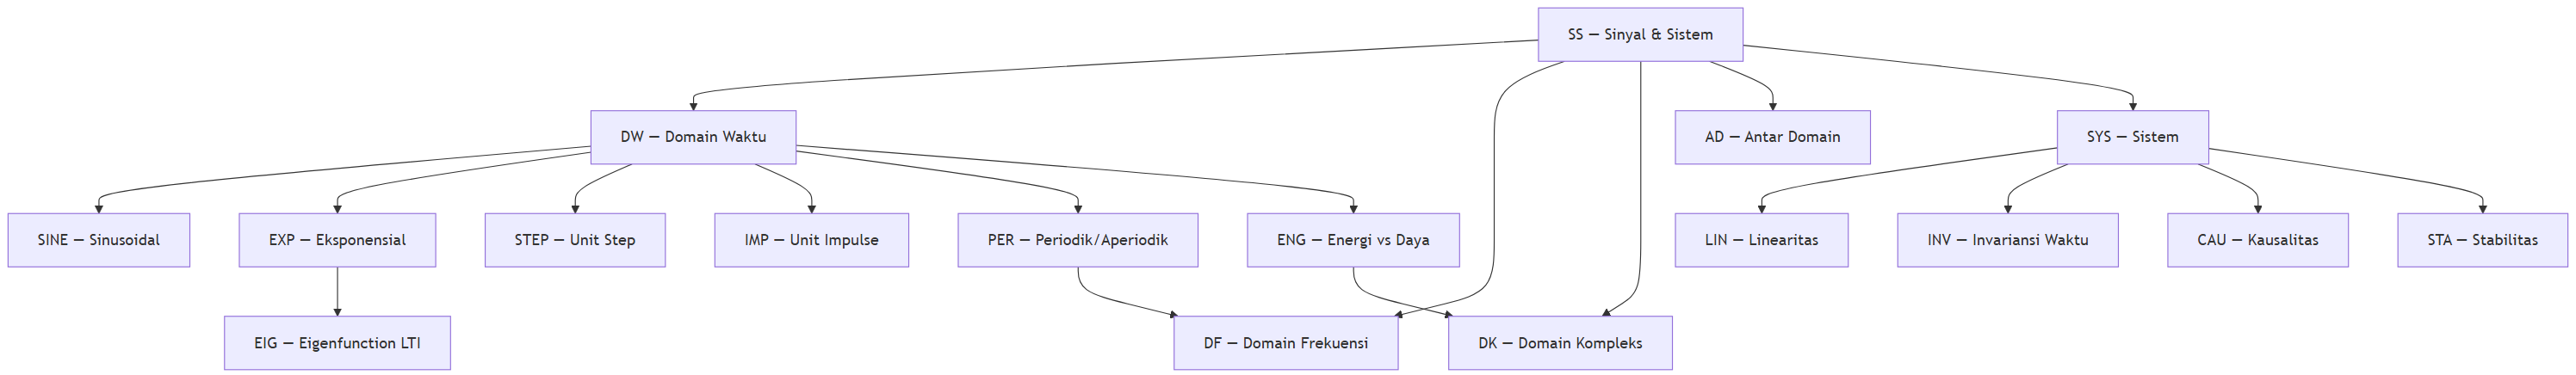
\includegraphics[width=27.12in,height=3.98in]{kuliah/Peta_1_files/figure-latex/mermaid-figure-1.png}

\begin{center}\rule{0.5\linewidth}{0.5pt}\end{center}

\bookmarksetup{startatroot}

\chapter{📘 Soal dari Oppenheim}\label{soal-dari-oppenheim}

\subsection{Soal 1}\label{soal-1}

\textbf{PN: OP-DW-SIGNAL-01-R} Sebutkan 4 contoh sinyal waktu-kontinu
dasar. ??? \textbf{Jawaban \& Penjelasan}: Eksponensial, sinusoidal,
unit step, unit impulse. Ini dasar untuk membangun sinyal kompleks.

\begin{center}\rule{0.5\linewidth}{0.5pt}\end{center}

\subsection{Soal 2}\label{soal-2}

\textbf{PN: OP-DW-SIGNAL-02-U} Jelaskan sifat eksponensial kompleks
\(e^{st}\). ??? \textbf{Jawaban \& Penjelasan}: Eksponensial kompleks =
eigenfunction sistem LTI. Jika \(s=j\omega\) → sinusoidal. Sifat ini
dasar Fourier/Laplace.

\begin{center}\rule{0.5\linewidth}{0.5pt}\end{center}

\subsection{Soal 3}\label{soal-3}

\textbf{PN: OP-DW-SIGNAL-03-A} Apakah \(x(t)=\sin(3t)+\cos(5t)\)
periodik? ??? \textbf{Jawaban \& Penjelasan}: Tidak periodik, karena 3/5
bukan bilangan rasional. Periodisitas butuh rasio frekuensi rasional.

\begin{center}\rule{0.5\linewidth}{0.5pt}\end{center}

\subsection{Soal 4}\label{soal-4}

\textbf{PN: OP-DW-SIGNAL-04-A} Hitung energi sinyal \(x(t)=e^{-t}u(t)\).
\emph{(Bloom: Apply)}

??? \textbf{Jawaban \& Penjelasan}:
\(E=\int_0^\infty e^{-2t} dt = 1/2\). Energi terbatas → sinyal energi,
bukan daya.

\begin{center}\rule{0.5\linewidth}{0.5pt}\end{center}

\section{🛠️ Peta Pemecahan Masalah -- Soal
4}\label{peta-pemecahan-masalah-soal-4}


\includegraphics[width=25.13in,height=5.33in]{kuliah/Peta_1_files/figure-latex/mermaid-figure-4.png}

\begin{center}\rule{0.5\linewidth}{0.5pt}\end{center}

\subsection{Soal 5}\label{soal-5}

\textbf{PN: OP-DW-SYSTEM-05-A} Apakah sistem \(y(t)=[x(t)]^2\) linear?
\emph{(Bloom: Apply)}

??? \textbf{Jawaban \& Penjelasan}: Tidak linear.

\begin{itemize}
\tightlist
\item
  Homogenitas gagal: \([a·x]^2 = a^2[x]^2 \neq a[x]^2\).
\item
  Aditivitas gagal: \([x₁+x₂]^2 \neq x₁²+x₂²\).
\end{itemize}

\begin{center}\rule{0.5\linewidth}{0.5pt}\end{center}

\section{🛠️ Peta Pemecahan Masalah -- Soal
5}\label{peta-pemecahan-masalah-soal-5}


\includegraphics[width=25.13in,height=5.33in]{kuliah/Peta_1_files/figure-latex/mermaid-figure-3.png}

\begin{center}\rule{0.5\linewidth}{0.5pt}\end{center}

\subsection{Soal 6}\label{soal-6}

\textbf{PN: OP-DW-SYSTEM-06-A} Apakah sistem \(y(t)=x(t-2)\) kausal? ???
\textbf{Jawaban \& Penjelasan}: Ya, output di t hanya bergantung input
waktu lampau/bersamaan.

\begin{center}\rule{0.5\linewidth}{0.5pt}\end{center}

\subsection{Soal 7}\label{soal-7}

\textbf{PN: OP-DW-SYSTEM-07-An}\\
Apakah sistem (y(t)=t \cdot x(t)) time-invariant?\\
\emph{(Bloom: Analyze)}

??? \textbf{Jawaban \& Penjelasan}:\\
Tidak time-invariant.\\
- Tes pergeseran:\\
Input digeser → (x(t-t₀)).\\
Output seharusnya (t·x(t-t₀)).\\
- Tetapi sistem memberi hasil: ((t-t₀)·x(t-t₀)).\\
- Karena hasil berbeda → sistem \textbf{time-varying}.

\begin{center}\rule{0.5\linewidth}{0.5pt}\end{center}

\section{🛠️ Peta Pemecahan Masalah -- Soal
7}\label{peta-pemecahan-masalah-soal-7}


\includegraphics[width=25.13in,height=5.33in]{kuliah/Peta_1_files/figure-latex/mermaid-figure-2.png}

\begin{center}\rule{0.5\linewidth}{0.5pt}\end{center}

\subsection{Soal 8}\label{soal-8}

\textbf{PN: OP-DW-SYSTEM-08-E} Apakah sistem
\(y(t)=\int_{-\infty}^t x(\tau)d\tau\) stabil? ??? \textbf{Jawaban \&
Penjelasan}: Tidak stabil. Input terbatas bisa hasilkan integral tak
terbatas (BIBO gagal).

Mantap. Ini \textbf{tambahan slide} untuk \textbf{Stabilitas (Soal 8:
integrator)}---lengkap dengan \textbf{peta pemecahan masalah}. Tempelkan
blok berikut ke file \texttt{.qmd} kamu (saya menaruhnya setelah Soal
8).

\section{````markdown}\label{markdown}

\subsection{Soal 8}\label{soal-8-1}

\textbf{PN: OP-DW-SYSTEM-08-E}\\
Apakah sistem ( y(t)=\displaystyle\int\_\{-\infty\}\^{}t x(\tau),d\tau )
\textbf{stabil (BIBO)}?\\
\emph{(Bloom: Evaluate)}

??? \textbf{Jawaban \& Penjelasan (ringkas \& ketat)}\\
- Uji BIBO via respon impuls: (h(t)=u(t)).\\
BIBO stabil ⇔ (\int\emph{\{-\infty\}\^{}\{\infty\}
\textbar h(t)\textbar,dt = \int\emph{0\^{}\{\infty\} 1,dt = \infty) →
\textbf{tidak stabil}.\\
- Kontra-contoh input terbatas: (x(t)=u(t)) (terbatas,
(\textbar x\textbar{}\le 1)).\\
Maka (y(t)=\int}\{-\infty\}\^{}t x(\tau),d\tau =
\int}\{0\}\^{}\{t\}1,d\tau = t) → \textbf{tak terbatas} saat
(t\to\infty).\\
Kesimpulan: \textbf{Tidak BIBO-stable}.

\begin{center}\rule{0.5\linewidth}{0.5pt}\end{center}

\section{🛠️ Peta Pemecahan Masalah -- Soal 8 (Stabilitas
Integrator)}\label{peta-pemecahan-masalah-soal-8-stabilitas-integrator}

\begin{Shaded}
\begin{Highlighting}[]
\NormalTok{flowchart TD}
\NormalTok{    A[Titik Mulai:\textless{}br/\textgreater{}S: y(t)= ∫\_\{{-}∞\}\^{}t x(τ)dτ]:::start}

\NormalTok{    \%\% Dua jalur uji stabilitas}
\NormalTok{    A {-}{-}\textgreater{} B[Definisi BIBO:\textless{}br/\textgreater{}Input terbatas ⇒ Output terbatas?]:::rule}
\NormalTok{    B {-}{-}\textgreater{} C1[Metode 1 – Uji ‖h‖₁:\textless{}br/\textgreater{}h(t)=u(t)]:::vehicle}
\NormalTok{    C1 {-}{-}\textgreater{} C2[Hitung ∫|h(t)|dt = ∫₀\^{}∞ 1 dt = ∞]:::calc}
\NormalTok{    C2 {-}{-}\textgreater{} C3[‖h‖₁ divergen ⇒ Tidak stabil]:::fail}

\NormalTok{    B {-}{-}\textgreater{} D1[Metode 2 – Kontra{-}Contoh:\textless{}br/\textgreater{}Pilih input terbatas]:::vehicle}
\NormalTok{    D1 {-}{-}\textgreater{} D2[x(t)=u(t), |x(t)|≤1]:::example}
\NormalTok{    D2 {-}{-}\textgreater{} D3[y(t)=∫₀\^{}t 1 dτ = t]:::calc}
\NormalTok{    D3 {-}{-}\textgreater{} D4[t → ∞ ⇒ y(t) tak terbatas]:::fail}

\NormalTok{    \%\% Kesimpulan}
\NormalTok{    C3 {-}{-}\textgreater{} K[Kesimpulan:\textless{}br/\textgreater{}Sistem TIDAK BIBO{-}Stable]:::conclusion}
\NormalTok{    D4 {-}{-}\textgreater{} K}

\NormalTok{    \%\% Styles}
\NormalTok{    classDef start fill:\#ffe082,stroke:\#333,stroke{-}width:2px}
\NormalTok{    classDef rule fill:\#e1f5fe,stroke:\#333,stroke{-}width:1px}
\NormalTok{    classDef vehicle fill:\#bbdefb,stroke:\#333,stroke{-}width:1px}
\NormalTok{    classDef calc fill:\#c8e6c9,stroke:\#333,stroke{-}width:1px}
\NormalTok{    classDef example fill:\#f3e5f5,stroke:\#333,stroke{-}width:1px}
\NormalTok{    classDef fail fill:\#ffcdd2,stroke:\#333,stroke{-}width:2px}
\NormalTok{    classDef conclusion fill:\#ffccbc,stroke:\#333,stroke{-}width:2px}
\end{Highlighting}
\end{Shaded}

\begin{center}\rule{0.5\linewidth}{0.5pt}\end{center}

\subsection{Soal 9}\label{soal-9}

\textbf{PN: OP-AD-09-An} Bandingkan representasi sinyal periodik di
domain waktu vs frekuensi. ??? \textbf{Jawaban \& Penjelasan}:

\begin{itemize}
\tightlist
\item
  Waktu: kombinasi sinus/cos.
\item
  Frekuensi: spektrum garis (impuls di harmonik).
\end{itemize}

\begin{center}\rule{0.5\linewidth}{0.5pt}\end{center}

\subsection{Soal 10}\label{soal-10}

\textbf{PN: OP-AD-10-C} Tuliskan representasi sinusoidal dalam bentuk
eksponensial kompleks. ??? \textbf{Jawaban \& Penjelasan}:
\(\cos(\omega t)=\tfrac{1}{2}(e^{j\omega t}+e^{-j\omega t})\). Dasar
transformasi Fourier.

\begin{center}\rule{0.5\linewidth}{0.5pt}\end{center}

\bookmarksetup{startatroot}

\chapter{📗 Soal dari Schaum's Outline}\label{soal-dari-schaums-outline}

\subsection{Soal 11}\label{soal-11}

\textbf{PN: SC-DW-SIGNAL-11-R} Definisikan sinyal energi dan sinyal
daya. ??? \textbf{Jawaban \& Penjelasan}: Energi:
\(E=\int |x(t)|^2dt<\infty\). Daya:
\(P=\lim_{T\to\infty}\frac{1}{2T}\int |x(t)|^2dt<\infty\).

\begin{center}\rule{0.5\linewidth}{0.5pt}\end{center}

\subsection{Soal 12}\label{soal-12}

\textbf{PN: SC-DW-SIGNAL-12-U} Apa arti penskalaan waktu \(x(at)\)? ???
\textbf{Jawaban \& Penjelasan}: \(a>1\) → kompresi waktu; \(0<a<1\) →
peregangan. Digunakan untuk analisis skala sinyal.

\begin{center}\rule{0.5\linewidth}{0.5pt}\end{center}

\subsection{Soal 13}\label{soal-13}

\textbf{PN: SC-DW-SIGNAL-13-A} Apakah \(x[n]=(-1)^n\) periodik? ???
\textbf{Jawaban \& Penjelasan}: Ya, periodik dengan N=2. Setiap dua
sampel pola berulang.

\begin{center}\rule{0.5\linewidth}{0.5pt}\end{center}

\subsection{Soal 14}\label{soal-14}

\textbf{PN: SC-DW-SIGNAL-14-A} Sketsa \(x(t)=u(t)-u(t-2)\). ???
\textbf{Jawaban \& Penjelasan}: Pulsa kotak: aktif 0 ≤ t \textless{} 2,
amplitudo = 1. Contoh sinyal diskrit dalam domain waktu.

\begin{center}\rule{0.5\linewidth}{0.5pt}\end{center}

\subsection{Soal 15}\label{soal-15}

\textbf{PN: SC-DW-SIGNAL-15-A} Hitung energi sinyal
\(x[n]=(1/2)^n u[n]\). ??? \textbf{Jawaban \& Penjelasan}:
\(E=\sum_{n=0}^\infty (1/4)^n=4/3\). Sinyal energi dengan energi
terbatas.

\begin{center}\rule{0.5\linewidth}{0.5pt}\end{center}

\subsection{Soal 16}\label{soal-16}

\textbf{PN: SC-DW-SYSTEM-16-A} Apakah sistem \(y[n]=x[n]+3\) linear? ???
\textbf{Jawaban \& Penjelasan}: Tidak linear karena ada offset
konstanta.

\begin{center}\rule{0.5\linewidth}{0.5pt}\end{center}

\subsection{Soal 17}\label{soal-17}

\textbf{PN: SC-DW-SYSTEM-17-An} Apakah sistem \(y[n]=x[-n]\)
time-invariant? ??? \textbf{Jawaban \& Penjelasan}: Ya, pembalikan
indeks berlaku konsisten jika input digeser.

\begin{center}\rule{0.5\linewidth}{0.5pt}\end{center}

\subsection{Soal 18}\label{soal-18}

\textbf{PN: SC-DW-SYSTEM-18-E} Apakah sistem
\(y[n]=\sum_{k=-\infty}^n x[k]\) stabil? ??? \textbf{Jawaban \&
Penjelasan}: Tidak stabil, akumulasi input terbatas bisa divergen.

\begin{center}\rule{0.5\linewidth}{0.5pt}\end{center}

\subsection{Soal 19}\label{soal-19}

\textbf{PN: SC-AD-19-An} Analisis perbedaan representasi sinyal di
domain waktu vs frekuensi. ??? \textbf{Jawaban \& Penjelasan}: Waktu →
bentuk sinyal. Frekuensi → distribusi energi/komponen. Saling
melengkapi.

\begin{center}\rule{0.5\linewidth}{0.5pt}\end{center}

\subsection{Soal 20}\label{soal-20}

\textbf{PN: SC-AD-20-C} Buat sistem diskrit yang \textbf{non-linear} dan
\textbf{tidak kausal}. ??? \textbf{Jawaban \& Penjelasan}:
\(y[n]=[x[n]]^2 + x[n+1]\). Non-linear (kuadrat), tidak kausal (butuh
input masa depan).

\begin{center}\rule{0.5\linewidth}{0.5pt}\end{center}

\bookmarksetup{startatroot}

\chapter{}\label{section}

\bookmarksetup{startatroot}

\chapter{Summary}\label{summary}

In summary, this book has no content whatsoever.

\bookmarksetup{startatroot}

\chapter*{References}\label{references}
\addcontentsline{toc}{chapter}{References}

\markboth{References}{References}

\phantomsection\label{refs}




\end{document}
